\documentclass[mphy386-notes.tex]{subfiles}
\begin{document}
\section{X-ray Image Quality}
In this section we will introduce the basics of x-ray imaging and develop three
tools that we can use to quantify image quality---contrast, resolution, and
noise. We will focus on x-ray imaging in these notes, but these tools are
useful for analyzing all imaging modalities.

\subsection{X-ray Imaging Basics}
We can create an x-ray imaging system by assembling an x-ray \textbf{source}, an
\textbf{object}, and a \textbf{detector}. Figure \ref{fig:simple} shows a simple
example of an x-ray imaging system---we place an x-ray fluence $\bs{\phi}_0$
incident on an object with two attenuation coefficients $\mu_1$ and $\mu_2$. Note that we use bold symbols to indicate random variables.
\begin{figure}[h]
\begin{center}
  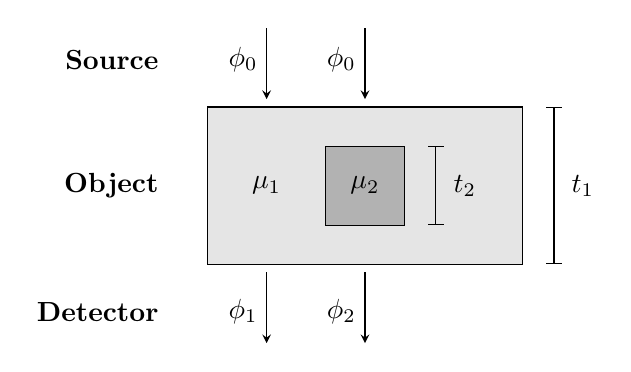
\begin{tikzpicture}[>=stealth]
    \filldraw[fill=black!10!white, draw=black] (-2,-1) rectangle (2,1);
    \filldraw[fill=black!30!white, draw=black] (-0.5,-0.5) rectangle (0.5,0.5);
    \draw [|-|] (2.4,-1) -- (2.4,1);
    \draw [|-|] (0.9,-0.5) -- (0.9,0.5);
    \node[right] at (1.0,0) {$t_2$};
    \node[right] at (2.5,0) {$t_1$};
    \node at (0,0) {$\mu_2$};
    \node at (-1.25,0) {$\mu_1$};
    \draw [->] (-1.25,2) -- (-1.25,1.1);
    \draw [->] (0,2) -- (0,1.1);
    \node at (-1.55,1.6) {$\bs{\phi}_0$};
    \node at (-.3,1.6) {$\bs{\phi}_0$};    
    \draw [->] (-1.25,-1.1) -- (-1.25,-2);
    \draw [->] (0,-1.1) -- (0,-2);
    \node at (-1.55,-1.6) {$\bs{\phi}_1$};
    \node at (-.3,-1.6) {$\bs{\phi}_{2}$};
    \node[left] at (-2.5, 1.6) {\textbf{Source}};
    \node[left] at (-2.5, 0) {\textbf{Object}};
    \node[left] at (-2.5, -1.6) {\textbf{Detector}};    
\end{tikzpicture}
\end{center}
\captionsetup{width=1.0\linewidth}
\caption{Simplified x-ray imaging schematic. A collimated beam of x-rays with
  fluence $\bs{\phi}_o$ is incident on an object with two attenuation
  coefficients. A detector measures the output fluences $\bs{\phi}_{1,2}$.}
\label{fig:simple}
\end{figure}
X-rays are attenuated as they pass through the object so the exit fluences are
related to the input fluence by
\begin{align}
  \bs{\phi}_1 &= \bs{\phi}_0e^{-\mu_1 t_1}\\
  \bs{\phi}_2 &= \bs{\phi}_0e^{-\mu_1(t_1 - t_2) - \mu_2t_2}. 
\end{align}
When we place a detector in the path of the exit beam we create an image of the
object. 

We will examine more realistic sources and detectors in later sections, but the
simple example in Figure \ref{fig:simple} is sufficient for us to model image
quality in x-ray imaging systems. 

\subsection{Rose Model}
Suppose that we'd like to detect the presence or absence of the small object
with attenuation $\mu_2$ in Figure \ref{fig:simple} with our imaging system. How
well can we perform this task? What conditions do we need to meet to confidently
say that the object is present or absent? How should we design our imaging
system to meet these conditions? The Rose model supplies answers to these
questions and gives us a solid framework for understanding image quality.

First, we define the \textbf{signal} $S$ as the mean number of photons
blocked by the object
\begin{align}
  S \equiv A(\text{E}\{\bs{\phi}_1\} - \text{E}\{\bs{\phi}_2\}) = A\Delta\phi
\end{align}
where $A$ is the cross sectional area of the object, $\text{E}\{\cdot\}$ denotes
the expectation value, $\phi$ is the x-ray fluence in units of photons per unit
area, and $\Delta\phi \equiv \text{E}\{\bs{\phi}_1\} -
\text{E}\{\bs{\phi}_2\}$. This may seem like a peculiar way to define the
signal---shouldn't the signal be the measured intensity difference between areas
with and without the object? The reason for our definition is that it captures
the role of object size in detectability. Intuitively, larger objects are easier
to detect, so our definition of signal should reflect this.

Next, we consider the \textbf{noise} $N$ that corrupts our signal. Note that in
signal-to-noise ratio discussions the word ``noise'' usually refers to the
standard deviation of a random variable. We will use this meaning. In general
the word ``noise'' refers to any random or unwanted signals.

We define the noise as the standard deviation of the number of photons detected
in an area the size of the object when the object is absent. 
\begin{align}
  N &\equiv \sqrt{\text{Var}\{A\bs{\phi}_1\}}.\\
  \intertext{$A\bs{\phi}_1$ is a Poisson-distributed random variable, so its variance is identical to its mean}
  N &= \sqrt{\text{E}\{A\bs{\phi}_1\}}\\
  N &= \sqrt{A\text{E}\{\bs{\phi}_1\}}.
\end{align}

Finally, the signal-to-noise ratio is given by
 \begin{align}
   \text{SNR} &\equiv \frac{S}{N} = \frac{A\Delta\phi}{\sqrt{AE\{\bs{\phi}_1\}}}
 \end{align}   
% %  \text{SNR} &= C\sqrt{A\bar{\phi}} 
% ^ is there a reason you've left this out?
 
where $C$ is the radiation contrast:
\begin{align}
  C = \frac{\Delta\phi}{\bar{\phi}}
\end{align}
This is the SNR for an ideal detector where we've assumed that there is
\begin{itemize}
\item complete absorption of incident quanta
\item no added noise
\item no loss of spatial resolution (i.e., no blurring)
\end{itemize}

\fig{img/contrast.png}{.25}{Test}{constrast}

\subsection{Linear Systems Model}

In this section, we aim to devise a mathematical model to
describe transmission radiography. Specifically, we would like to
use linear systems theory to describe the final radiographic
image as a convolution of the object with a point spread function (PSF)
contributed by both the x-ray source and the detector.

To begin, we consider a simplified geometric representation of an x-ray
system, shown in Figure~\ref{fig:xraymodel}:

\fig{img/xraymodel.png}{0.65}{Simplified geometry of a radiographic
  imaging system. Note: we will refer to the central plane as the
``object plane,'' not ``aperture plane,'' as it appears here.}{xraymodel}

X-rays are generated at the anode of an x-ray tube, located in the
\textbf{source plane} (with coordinate $\bs{r}$). They then pass through the
\textbf{object plane} (with coordinate $\bs{r}'$), before
being detected at the \textbf{detector plane} (with coordinate $\bs{r}''$).
The distance between the source and object planes is $s_1$, and the distance
between the object and detector planes is $s_2$. Clearly, there are a number
of idealizations in this setup. We model the 3D anode and 3D object as
2D planes, and assume that all three planes are parallel. Regardless,
we can still draw important insights from this simplified model.

\subsubsection{The Source}

We describe the source by an \textit{emission function} $f(\bs{r})$, where
$\bs{r}$ is the two-dimensional vector in the source plane. The emisison
function has units of fluence rate: (photons / unit time $\cdot$ unit
area). Thus, the quantity $f(\bs{r})d^2 r$ is the \textit{mean} number of
photons per unit time emitted into all space from an elemental area $d^2 r$
located at the point $\bs{r}$. Note that this introduces another assumption that
the source emits photons isotropically. In fact, bremsstrahlung photons have
a definite preferred orientation which depends on electron energy, angle of
electron incidence, and target material.

\fig{img/solidangle}{0.65}{Diagram for solid-angle calculation.}{solidangle}

\subsubsection{The Detector}

Now, let us consider an elemental detector of area $d^2\bs{r}''$, where
$\bs{r}''$ is the two-dimensional position vector in the detector plane.
We can calculate the solid angle $d\Omega$ subtended by the elemental
detector area from the source as:
\begin{align}
  d\bs{\Omega} = \frac{d^2\bs{r}''\cdot\text{cos}\theta}{R^2},
  \label{eq:sa}
\end{align}
where $R$ is the distance from the source element to the detector element and
$\theta$ is the angle between the normal to the detector surface and the line of
sight from source to detector, as shown in Figure~\ref{fig:solidangle}. From
simple geometry, we know that
\begin{align}
  R = (s_1 + s_2) / \text{cos}\theta,
\end{align}
so we can rewrite Equation~\ref{eq:sa} as
\begin{align}
  d\bs{\Omega} = \frac{\text{cos}^3\theta}{(s_1 + s_2)^2}d^2\bs{r}''.
\end{align}

Since a full sphere subtends $4\pi$ steradians, the detector element would
intercept a fraction $d\bs{\Omega}/4\pi$ of the radiation emitted from
any source element in the absence of absorbing material in between
the source and detector planes. In this case, the mean number of
photons per unit time (1) emitted by the area element $d^2\bs{r}$ in the source
plane and (2) intercepted by the area element $d^2\bs{r}''$ in the detector
plane would be
\begin{align}
  f(\bs{r})d^2\bs{r}\frac{d\bs{\Omega}}{4\pi} = f(\bs{r})\frac{\text{cos}^3\theta}{4\pi(s_1+s_2)^2}d^2\bs{r}d^2\bs{r}''.
\end{align}

For now, we are assuming an ideal, continuous detector that detects all photons
that intercept it. We will lift this restriction shortly; in general, we will
see that the detector should be considered an integral part of the imaging
system.

\subsubsection{The Object Plane}

We now consider the effect of the object. We introduce another restriction
that we are only dealing with \textit{primary} x-rays; we will discuss the
effect of scattered radiation later. A ray emanating from point $\bs{r}$ and
striking the detector at point $\bs{r}''$ will have passed through the object
plane at point $\bs{r}'$. We define $g(\bs{r}')$ as the transmittance, or the
fraction of photons that pass through the object plane at point $\bs{r}'$.

We are now in a position to write down an expression for $h(\bs{r}'')$, the
density of detected photons, such that $h(\bs{r}'')d^2\bs{r}''$ is the mean
number of photons intercepted by the detector area $d^2\bs{r}''$ in a time T.
We are not interested in where exactly in the source the photons come from,
so we integrate over the entire source plane:
\begin{align}
  h(\bs{r}'')d^2\bs{r}'' = \frac{Td^2\bs{r}''}{4\pi(s_1 + s_2)^2}\int_{\text{source}}d^2\bs{r} \text{ cos}^3\theta f(\bs{r})g(\bs{r}').
  \label{eq:h1}
\end{align}
$h(\bs{r}'')$ has dimensions of fluence (photons per unit area), though
we refer to $h(\bs{r}'')$ as a \textit{photon density} instead, as that
term is more appropriate to a static pattern of recorded photons.

Looking closely at the geometry of Figure~\ref{fig:xraymodel}, we
see that
\begin{align}
  \frac{\bs{r}'-\bs{r}}{s_1} = \frac{\bs{r}''-\bs{r}'}{s_2},
  \label{eq:v1}
\end{align}
or, equivalently:
\begin{align}
  \bs{r}' = \frac{s_2}{s_1 + s_2}\bs{r} + \frac{s_1}{s_1+s_2}\bs{r}'' = a\bs{r}'' + b\bs{r},
  \label{eq:v2}
\end{align}
where
\begin{align}
  a = \frac{s_1}{s_1+s_2} & & b = \frac{s_2}{s_1 + s_2} = 1 - a,
\end{align}
and we have eliminated the vector $\bs{r}'$. Note that Equations~\ref{eq:v1}
and~\ref{eq:v2} describe 2D (not 3D!) vector subtractions in the parallel $(x,y)$
and $(x',y')$ planes. The 3D distance $R$ would be written
\begin{align}
  R = \sqrt{|\bs{r}-\bs{r}''|^2 + (s_1+s_2)^2}.
\end{align}
With this simplification, we can rewrite Equation~\ref{eq:h1} without the use of $\bs{r}'$ as
\begin{align}
  h(\bs{r}'')d^2\bs{r}'' = Cd^2\bs{r}''\int_{\text{source}}d^2\bs{r} \text{ cos}^3\theta f(\bs{r})g(a\bs{r}'' + b\bs{r}),
\end{align}
where
\begin{align}
  C = \frac{T}{4\pi(s_1+s_2)^2}.
\end{align}
We are generally interested in systems where $s_1 + s_2$ is large compared to $|\bs{r}|$ or $|\bs{r}''|$. We
can thus make the approximation $\theta \approx 0$ and $\text{cos}^3\theta \approx 1$. Dropping the
$d^2\bs{r}''$ factor from both sides, this leaves us with our final model for the density of detected
photons:
\begin{align}
  h(\bs{r}'') \approx C\int_{source}d^2 \bs{r} f(\bs{r})g(a\bs{r}'' + b\bs{r}).
  \label{eq:hfinal}
\end{align}

It is important to keep track of the various assumptions we used to build this model.
To summarize, we assume:
\begin{itemize}
\item we have a 2D, planar, isotropic source that is far from the detector plane ($\theta\approx 0$)
\item we have a 2D planar object that does not introduce scattered radiation
\item we have an ideal detector that perfectly detects every photon it encounters
\end{itemize}

\subsubsection{Reduction to a Convolution}

Equation~\ref{eq:hfinal} is starting to resemble a convolution integral. To exploit this
resemblance, we define a new variable $\bs{r}_0''$, given by
\begin{align}
  \bs{r}_0'' = \frac{s_2}{s_1}\bs{r} = -\frac{b}{a}\bs{r}.
\end{align}
Multiplication of $\bs{r}$ by $-b/a$ is equivalent to projecting it through a
point in the object plane to the image plane, as illustrated in Figure~\ref{fig:r0}.

\fig{img/r0}{0.5}{Illustration of $\bs{r}_0''$.}{r0}

We can use $\bs{r}_0''$ to define scaled versions of $f$ (the source emittance)
and $g$ (the object transmittance).  We define these scaled functions as
$\tilde{f}$ and $\tilde{g}$, respectively:
\begin{align}
  \tilde{f}(\bs{r}_0'') &= f(\bs{r}) = f\left(-\frac{a}{b}\bs{r}_0''\right)\\
  \tilde{g}(\bs{r}_0'') &= g(a\bs{r}_0'').
\end{align}

The tilde thus indicates \textit{projection of the initial functions onto the image plane}. We
can rewrite $g$ in terms of these new variables: 
\begin{align}
  g(a\bs{r}'' + b\bs{r}) = g(a\bs{r}''-a\bs{r}_0'') = \tilde{g}(\bs{r}'' - \bs{r}_0''),
\end{align}
which leads to a final form for $h(\bs{r}'')$:
\begin{align}
  h(\bs{r}'')&=\left(\frac{a}{b}\right)^2 C \int_{\infty} d^2\bs{r}_0'' \tilde{f}(\bs{r}_0'')\tilde{g}(\bs{r}'' - \bs{r}_0'')\nonumber\\
             &=\left(\frac{a}{b}\right)^2 C \tilde{f}(\bs{r}'') \ast \ast \text{ } \tilde{g}(\bs{r}'')
\end{align}
where the $\infty$ subscript in the integral indicates integration over the
entire 2D detector plane. We have thus achieved our goal and described the
detected photon density as the output of a 2D linear system with input
$\tilde{f}$ and kernel proportional to $\tilde{g}$ (or equivalently, an input
$\tilde{g}$ and kernel proportional to $\tilde{f}$). As with any linear system, a
frequency-domain description is very useful:
\begin{align}
  \mathscr{F}_2\left\{h(\bs{r}'')\right\} = H(\bs{\rho}'') = (a/b)^2 C \tilde{F}(\bs{\rho}'')\tilde{G}(\bs{\rho}),
  \label{eq:ft1}
\end{align}
where $\bs{\rho}''$ is the spatial frequency vector conjugate to $\bs{r}''$ in the image plane.
Recall the scaling relation for an nD Fourier transform:
\begin{align}
  \mathscr{F}_N\left\{f(\bs{r}/b)\right\} = |b|^N F(b\bs{\rho}).
\end{align}
We can use this to evaluate the right side of Equation~\ref{eq:ft1} in terms of the
original source and transmission functions $f$ and $g$:
\begin{align}
  \tilde{F}(\bs{\rho}'') &= \mathscr{F}_2\left\{f(-a\bs{r}''/b)\right\} = (b/a)^2 F(-b\bs{\rho}''/a)\\
  \tilde{G}(\bs{\rho}'') &= \mathscr{F}_2\left\{g(a\bs{r}'')\right\} = (1/a)^2 G(\bs{\rho}''/a).
\end{align}
Our final result is then
\begin{align}
  H(\bs{\rho}'') = (C/a^2)F(-b\bs{\rho}''/a)G(\bs{\rho}''/a).
  \label{eq:ft2}
\end{align}

Recall that the double-primed coordinate represent the frequency vector
in the image plane. We can also express Equation~\ref{eq:ft2} in the
object ($\bs{\rho}'$) and source ($\bs{\rho}$) planes:
\begin{align}
  H(a\bs{\rho}') &= (C/a^2)F(-b\bs{\rho}')G(\bs{\rho}')\\
  H(-a\bs{\rho}/b) &= (C/a^2)F(\bs{\rho})G(-\bs{\rho}/b).
\end{align}

\subsubsection{Effect of focal spot}

The perhaps non-intuitive result of this analysis is that the x-ray source plays
such an important role in the imaging chain. We have shown that the detected
image can be modeled as a convolution of the object with the x-ray source -- the
source is thus always ``in'' the image, in a certain sense. We would like to
characterize this effect in more detail.

We can model the x-ray source as a ``focal spot,'' a uniform, emissive disk of
diameter $d_{fs}$, so the emission function is
\begin{align}
  f(\bs{r}) = f_0 \text{ circ}\left(\frac{2r}{d_{fs}}\right),
  \label{eq:fsdef}
\end{align}
where $f_0$ is the emission density (photons per unit area per unit time) within
the disk region (see Figure \ref{fig:fs}). Recall that the ``circ'' function is
defined as:
\begin{align}
  \text{circ}(r) =
  \begin{cases}
    1 & r \le 1\\
    0 & \text{else}
  \end{cases}.
\end{align}

\fig{img/focal_spot}{0.75}{Diagram illustrating the calculation of the point
  spread function for transmission radiography with a disklike focal spot.}{fs}

To find the PSF of the system, we consider a point
object input described by
\begin{align}
  g(\bs{r}') = \delta(\bs{r}'-\bs{r}_1'),
  \label{eq:pinhole}
\end{align}
where $\bs{r}_1'$ is the location of the point in the object plane. The notion
of a ``point'' transmission might seem counterintuitive -- we are describing a
hypothetical object that becomes ``infinitely transmissive'' over an
infinitesimal area. You might consider a pinhole aperture with area
approaching zero while the exposure time is increased proportionally.

The PSF is just the image of a point source measured in the detector plane --
i.e., the pinhole image of the focal spot. Substituting Equations~\ref{eq:fsdef}
and~\ref{eq:pinhole} into~\ref{eq:hfinal}, we find
\begin{align}
  h(\bs{r}'') &= C \int_{source} d^2\bs{r} f_0 \text{ circ} \left(\frac{2r}{d_{fs}}\right)\delta(a\bs{r}'' + b\bs{r}-\bs{r}')\nonumber\\[6pt]
              &= \left(\frac{C}{b^2}\right) f_0 \text{ circ}\left[\frac{2|a\bs{r}'' - \bs{r}_1'|}{bd_{fs}}\right]\nonumber\\[6pt]
              &= \left(\frac{C}{b^2}\right) f_0 \text{ circ}\left[\frac{2|\bs{r}''-(\bs{r}_1'/a)|}{b d_{fs} / a}\right],
\end{align}
where we have made use of the sifting property of delta functions. This equation
describes a uniform disk image of diameter $d_{fs}''$, given by
\begin{align}
  d_{fs}'' = \frac{b}{a}d_{fs} = \frac{s_2}{s_1}d_{fs}.
\end{align}
The disk is centered at $\bs{r}'' = \bs{r}_1'/a = \bs{r}_1'(s_1 + s_2)/s_1$, the
magnification $m_t$ is therefore $(s_1 + s_2)/s_1$. Note that $m_t$ is always a positive number greater than 1.

To completely specify the PSF we must also include the effects of the image
detector, which we have so far neglected. An ideal detector would produce output
directly proportional to $h(\bs{r''})$. Real detectors, however, further degrade
the image and must be treated as independent linear systems. Cascaded linear
systems are easiest to deal with in the frequency domain, so we consider the
input of the \textit{detector} system to be $H(\bs{\rho}'')$, the
Fourier transform of $h(\bs{r}'')$. We denote the transfer function of
the detector as $D(\bs{\rho}'')$, so the detector output is just
$D(\bs{\rho}'')H(\bs{\rho}'')$. Using Equation \ref{eq:ft2}, we can write this
as
\begin{align}
  D(\bs{\rho}'')H(\bs{\rho}'') = (C/a^2)D(\bs{\rho}'')F(-b\bs{\rho}''/a)G(\bs{\rho}''/a).
\end{align}

This describes the transfer of spatial frequencies $G(\bs{\rho}''/a)$, the
object function scaled into the detector plane. We are \textit{actually}
interested in how the spatial frequencies of the object in the \textit{object
  plane} (i.e., with no scaling) are affected by the system, so we let
$\bs{\rho}' = \bs{\rho}''/a$ and rewrite our result as
\begin{align}
  D(a\bs{\rho}')H(a\bs{\rho}') = (C/a^2)D(a\bs{\rho}')F(-b\bs{\rho}')G(\bs{\rho}').
\end{align}
Note that $G(\bs{\rho}')$ now appears on the right side with no scaling. The
overall transfer function of the system for spatial frequencies in the object
plane is thus given by
\begin{align}
  TF_{tot}(\bs{\rho}') = P_{tot}(\bs{\rho}') = (C/a^2)D(a\bs{\rho}')F(-b\bs{\rho}'),
  \label{eq:TFtot}
\end{align}
which we can write in the spatial domain as
\begin{align}
  \text{PSF}_{tot}(\bs{r}') &= p_{tot}(\bs{r}') = (C/a^2)\mathscr{F}_2^{-1}\left\{D(a\bs{\rho}')F(-b\bs{\rho}')\right\}\\
                               &= p_{fs}(\bs{r}') \ast \ast \text{ }p_{det}(\bs{r}'),
\end{align}
where $p_{fs}(\bs{r}')$ is the PSF due to the focal spot alone:
\begin{align}
  p_{fs}(\bs{r}') = (C/a^2)\mathscr{F}_2^{-1}\left\{F(-b\bs{\rho})\right\} = \left(\frac{C}{a^2b^2}\right)f\left(-\bs{r}'/b\right),
  \label{eq:psffs}
\end{align}
and $p_{det}(\bs{r}')$ is the PSF due to the detector:
\begin{align}
  p_{det}(\bs{r}') = \mathscr{F}_2^{-1}\left\{D(a\bs{\rho}')\right\} = (1/a^2)d\left(\bs{r}'/a\right).
  \label{eq:psfdet}
\end{align}

\subsubsection{Design Considerations}

We can now discuss how to use our results from the linear systems
model to optimize our imaging system design. Specifically, we see
that there is an optimum magnification even if there is no limitation
imposed by the finite detector size. Recall that the magnification is
given by
\begin{align}
  m_t = \frac{s_1+s_2}{s_1} = \frac{1}{a} = \frac{1}{1-b}.
  \label{eq:mag1}
\end{align}
Equivalently, we see that
\begin{align}
  b = 1 - \frac{1}{m_t} = \frac{m_t - 1}{m_t}.
  \label{eq:mag2}
\end{align}
Applying these results to Equations~\ref{eq:psffs} and~\ref{eq:psfdet},
we see that
\begin{align}
  p_{fs}(\bs{r}') &\propto f\left(\frac{-m_t\bs{r}'}{m_t - 1}\right)\label{eq:psffsmag}\\
  p_{det}(\bs{r}') &\propto d(m_t\bs{r}')\label{eq:psfdetmag}
\end{align}
The width of $p_{fs}(\bs{r}')$ is smallest when the coefficient of $\bs{r}'$ of
Equation~\ref{eq:psffsmag} is the largest, which occurs when $m_t = 1$. Blurring
from the focal spot is thus minimized for ``contact'' imaging ($s_2 = 0$), when
the detector is in direct contact with the object being imaged, and there is no
magnification. We see from Equation~\ref{eq:psfdetmag}, however, that a large
magnification is needed to minimize blurring from the detector.

To optimize the choice of magnification, then, we can model the PSFs from the
focal spot and detector as Gaussians. Recall that the Fourier transform of a
Gaussian function is another Gaussian function. In the frequency domain then, we
will assume that
\begin{align}
  D(\bs{\rho}'') &\propto \text{exp}\left[-\pi\left(\bs{\rho}''/\rho_d''\right)^2\right]\\
  F(\bs{\rho}) &\propto \text{exp}\left[-\pi\left(\bs{\rho}/\rho_f\right)^2\right],
\end{align}
where $\rho_d''$ and $\rho_f$ are characteristic widths of the MTF of the detector and
focal spot, respectively. We find the overall MTF from Equation~\ref{eq:TFtot},
\begin{align}
  \text{MTF}_{tot} = \frac{|P_{tot}(\bs{\rho}')|}{P_{tot}(0)} \propto \text{exp}\left[-\pi(a\bs{\rho}'/\rho_d'')^2\right]\text{exp}\left[-\pi(b\bs{\rho}'/\rho_f'')^2\right].
\end{align}
From Equations~\ref{eq:mag1} and~\ref{eq:mag2}, this can be written as
\begin{align}
  \text{MTF}_{tot} = \text{exp}\left[-\pi\bs{\rho}'\left(\frac{1}{(m_t \rho_d'')^2} + \frac{(m_t-1)^2}{(m_t\rho_f)^2}\right)\right].
\end{align}
The width of MTF$_{tot}$ will be an extremum if
\begin{align}
  \frac{d}{d m_t}\left[\frac{1}{(m_t \rho_d'')^2} + \frac{(m_t-1)^2}{(m_t\rho_f)^2}\right] = 0,
\end{align}
which has the solution
\begin{align}
  m_t^{opt} = 1 + \left(\frac{p_f}{p_d}\right)^2.
  \label{eq:magopt}
\end{align}

We are interested in two limits of Equation~\ref{eq:magopt}. If we have a very
large focal spot ($\rho_f \to 0$), then $m_t^{opt} = 1$, which, as we have already
discussed, indicates contact imaging. On the other hand, if our detector is very
poor ($\rho_d'' \to 0$), we require a large magnification. In other words, we can
tolerate having a large focal spot by performing contact imaging, at the cost of
having no magnification. This is generally what occurs, as the focal spot is
often a more dominant contribution to the system PSF than the detector.

Note: this discussion on linear systems theory was adapted from Chapter 4 in
Barrett~\cite{barrett}. Please read through the rest of that chapter for a more
detailed analysis and insight into further design considerations. 


\pagebreak
\end{document}